%!TEX root = ./book_omp.tex
% !TEX encoding = UTF-8 Unicode
%======================================================================================================================
% J.ROUSSEL
% 2019-09-11	 : création 
\setchapterstyle{kao}
\setchapterpreamble[u]{\margintoc}
\chapter{TRANSFORMÉE DE FOURIER}
\labch{TF}

% Introduction
Jusqu'à maintenant nous n'avons envisagé que des signaux périodiques dont nous avons mis en évidence la décomposition en série de Fourier, et où le poids de chaque harmonique se distribue selon un histogramme que l'on appelle spectre du signal. 

Hélas, certains signaux \emph{ne sont pas} périodiques. On peut penser aux impulsions lumineuses, au potentiel d'action d'une fibre nerveuse, au signal acoustique du langage etc. Les notions d'harmoniques et de spectre ont-ils encore un sens ? Ce chapitre répond à cette question et montre le rôle unificateur que joue la transformée de Fourier dans différents domaines de la physique.

\begin{center}
\textbf{Version en ligne}

	\url{https://femto-physique.fr/omp/transformee-de-fourier.php}
\end{center}

\section{Transformation de Fourier} % (fold)
\label{sec:transformee_de_fourier}

\subsection{Du discret au continu} % (fold)
\label{sub:spectre_continu}
Nous avons établi dans le chapitre  précédent que tout signal périodique physique peut s'écrire en notation complexe
\[
f_T(t)=\sum_{n=-\infty}^\infty \underline{c_n}\,\mathrm{e}^{i n\,2\pi\nu\,t}
\quad\text{avec}\quad
\nu=\frac{1}{T}
\]
où \({\underline{c_n}}\) est un ensemble \textbf{discret} de coefficients complexes donnés par
\[
\underline{c_n}=\frac{1}{T}\int_{-T/2}^{T/2}f(t) \, \mathrm{e}^{-i n\,2\pi\nu\, t}\,\mathrm{d}t
\quad\text{avec}\quad n\in \mathbb{Z}
\]
Considérons dorénavant un signal \(f(t)\) \textbf{non périodique}. On peut toujours considérer que le signal représente un unique motif d'un signal périodique dont la période tendrait vers l'infini. En d'autres termes, on peut considérer que le signal est de fréquence \(\nu\to 0\) et que les harmoniques balayent tout l'espace des réels ; le spectre discret devenant alors continu. Voyons comment cela se traduit mathématiquement. D'après les relations précédentes, un signal périodique peut s'écrire
\[
f_T(t)=\sum_{n=-\infty}^\infty \left[
\nu\int_{-T/2}^{T/2}f(t')\,\mathrm{e}^{-i n\,2\pi\nu\,t'}\,\mathrm{d}t'\right]\,\mathrm{e}^{i n\,2\pi\nu\,t}
\]
Faisons tendre \(T\to \infty\) c'est-à-dire \(\nu\to 0\) :
\[
	f(t)=\lim_{\nu\to 0} \sum_{n=-\infty}^\infty \left[
	\mathrm{e}^{i n\,2\pi\nu\,t} \int_{-\infty}^{\infty}f(t')\,\mathrm{e}^{-i n\,2\pi\nu\, t'}\,\mathrm{d}t'\right]\, \nu
\]
On reconnaît ici une intégrale au sens de Riemann\sidenote{Rappelons qu'une intégrale peut être vue comme une somme de rectangles sous la courbe avec un espacement tendant vers 0. Mathématiquement on a l'identité
\[
	\int_{-\infty}^\infty g(\nu)\, \mathrm{d}\nu=\lim_{\nu\to 0}\sum_{n=-\infty}^{\infty}g(n\nu)\nu
\]}. Ainsi, un signal non périodique peut formellement s'écrire
\[
	f(t)=\int_{-\infty}^\infty \mathrm{e}^{i2\pi\nu\, t} \left[\int_{-\infty}^{\infty}f(t')\,\mathrm{e}^{-i2\pi\nu\,t'}\,\mathrm{d}t'\right]\, \mathrm{d}\nu
\]
Le terme entre crochets est appelé \textbf{transformée de Fourier}.

\begin{kaobox}[frametitle=Intégrale de Fourier]
Tout signal physique\footnote{Précisément, on restreint l'étude à tous les signaux de carré sommable pour lesquelles \(\int_{\mathbb{R}}|f(t)|^2\,\mathrm{d}t\) est finie, c'est-à-dire des signaux qui transportent une énergie finie.} peut se décomposer en une intégrale  de Fourier, de la forme
\begin{equation}
f(t)=\int_{-\infty}^\infty \widehat{f}(\nu)\,\mathrm{e}^{i2\pi\,\nu\, t}\,\mathrm{d}\nu
\label{TFinverse}
\end{equation}
où \(\widehat{f}(\nu)\) désigne la transformée de Fourier du signal. \(\widehat{f}(\nu)\) est une fonction continue à valeurs complexes, définie par
\begin{equation}
	\widehat{f}(\nu)=\int_{-\infty}^{\infty}f(t)\,\mathrm{e}^{-i2\pi\,\nu\,t}\,\mathrm{d}t
	\label{TF}
\end{equation}
\end{kaobox}

La transformée de Fourier \(\widehat{f}(\nu)\) est une fonction continue de la fréquence et joue le même rôle que les coefficients de Fourier du signal périodique. La relation \eqref{TFinverse} peut s'interpréter comme une somme continue d'harmoniques complexes, la fonction \(\widehat{f}(\nu)\) traduisant le «poids relatif» des diverses fréquences.
\begin{marginfigure}[*1]
\centering
\begin{tikzpicture}[scale=1]
	\begin{axis}[
		height=4cm,
		width=6cm,
		axis lines=middle,% bottom,top
		inner axis line style={=>},
		xlabel style={anchor=west},
		ylabel style={anchor=west},
		xlabel={$t$},ylabel={$\Pi_\tau(t)$},
		ymin=0,ymax=1.25,xmin=-5,xmax=5,
		ytick={1},
		xtick={-1,1},xticklabels={\(-\frac{1}{2}\tau\),\(\frac{1}{2}\tau\)},
		font=\footnotesize,
		]
		\draw[thick,monBleu] (axis cs:-4,0)--(axis cs:-1,0)--(axis cs:-1,1)--(axis cs:1,1)--(axis cs: 1,0)--(axis cs:4,0);
	\end{axis}
\end{tikzpicture}
\caption{Fonction porte.}
\end{marginfigure}

\exercice{Calculer la transformée de Fourier d'une \emph{fonction porte} de largeur temporelle \(\tau\) définie par :
\[
	\Pi_\tau(t)=\begin{cases}
		1& \text{ si }|t|<\frac12 \tau\\
		0&\text{sinon}
	\end{cases}
\]
\\[2mm]
\emph{Rép. -- } \(\widehat{\Pi}_\tau(\nu)=\tau\, \text{sinc}(\pi\nu\tau)\)
}
Le graphe de \(|\widehat{f}|\) en fonction de la fréquence est appelé spectre d'amplitude du signal, alors que le graphe de \(|\widehat{f}|^2\) est son \emph{spectre en énergie}. Par exemple, la densité spectrale de puissance d'une fonction porte à la forme d'un sinus cardinal au carré (\emph{cf.} \reffig{Spectres_d_un_signal_rectangulaire}). On voit notamment qu'un tel signal contient des harmoniques dont les valeurs s'étendent jusqu'à l'infini. Toutefois, l'essentiel des harmoniques se situe dans un bande de fréquence définie par
\[
	|\nu|<\frac{1}{\tau}
\]
\begin{marginfigure}
	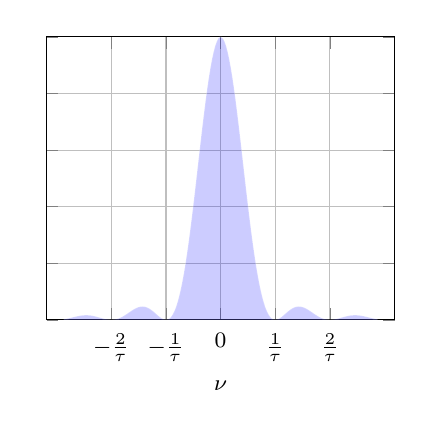
\begin{tikzpicture}
		\begin{axis}[
			width=6cm,
			grid=major,
			xlabel={\(\nu\)},
			xtick={-6.28,-3.14,0,3.14,6.28},
			xticklabels={\(-\frac{2}{\tau}\),\(-\frac{1}{\tau}\),0,\(\frac{1}{\tau}\),\(\frac{2}{\tau}\)},
			x tick label style={below=0.5mm},
			yticklabels=\empty,
			xmin=-10,
			xmax=10,
			ymin=0,
			ymax=1,
			font=\footnotesize,
			]
		\addplot+[draw=white,fill=blue,mark=none,opacity=0.2,domain=-9:9,samples=200]{(sin(x*180/pi)/x)^2}\closedcycle;
		\end{axis}
	\end{tikzpicture}
	\caption{Spectre en puissance d'une fonction porte de largeur temporelle \(\tau\).}
	\labfig{Spectres_d_un_signal_rectangulaire}
\end{marginfigure}
En d'autres termes, plus brève est l'impulsion, plus vaste est le domaine des harmoniques qui constitue le signal. De façon équivalente, plus courte est la résolution temporelle avec laquelle on veut analyser un signal plus large sera la bande passante de l'analyseur employée pour traiter le signal.

La relation de Parseval \(\overline{f^2}=\displaystyle\sum_{n=-\infty}^\infty |\underline{c_n}|^2\) rencontrée dans le \refch{serie-de-fourier} prend également une forme intégrale lors du passage au continu. On obtient
\begin{equation}
\fcolorbox{filet}{fond}{\hspace{0.5em}
\(\displaystyle
\int_{\mathbb{R}}|f(t)|^2\, \mathrm{d}t=\int_{\mathbb{R}}|\widehat{f}(\nu)|^2\, \mathrm{d}\nu
\)\hspace{0.5em}}
\hspace{0.5em}\heartsuit
\label{eq:relation_de_Parseval_Plancherel}
\end{equation}
Autrement dit, l'énergie totale d'un signal ne dépend pas de la représentation choisie : fréquentielle ou temporelle.

\exercice{Vérifier la relation \eqref{eq:relation_de_Parseval_Plancherel} sur l'exemple de la fonction porte sachant que
\[
	\int_{\mathbb{R}} \left(\frac{\sin x}{x}\right)^2\, \mathrm{d}x=\pi
\]}

\begin{kaoremark}
Certains préfèrent une décomposition spectrale en pulsation (\(\omega\)) plutôt qu'en fréquence (\(\nu\)). Dans ce cas les transformations de Fourier s'écrivent
\[
f(t)=\frac{1}{\sqrt{2\pi}}\int_{\mathbb{R}} \widehat{f}(\omega)\,\mathrm{e}^{i\,\omega t}\, \mathrm{d}\omega
\quad\text{avec}\quad
\widehat{f}(\omega)=\frac{1}{\sqrt{2\pi}}\int_{\mathbb{R}}f(t)\,\mathrm{e}^{-i\,\omega t}\,\mathrm{d}t
\]
\end{kaoremark}
% (end)
\subsection{Quelques propriétés de la Transformée de Fourier}[Quelques propriétés] % (fold)
\label{sub:proprietes_de_la_transformee_de_fourier}
On dit que \(f(t)\) et \(\widehat{f}(\nu)\) forment une paire de transformées de Fourier. On passe de l'une à l'autre par une transformation de Fourier (TF) ou transformation de Fourier inverse (TF\(^{-1}\)) :
\[
f(t) \quad\xrightleftharpoons[\text{TF}^{-1}]{\text{TF}}\quad \widehat{f}(\nu)
\]
Énonçons\sidenote[][*0]{On donne ici des résultats faciles à démontrer à partir des relations \eqref{TFinverse} et \eqref{TF}.} quelques propriétés de la transformée de Fourier des signaux réels :
\begin{description}
	\item[Linéarité --] En vertu de la linéarité de l'intégration, la transformation de Fourier est aussi une opération linéaire :
	\[
	a\,f(t)+b\,g(t)\quad\rightleftharpoons\quad a\,\widehat{f}(\nu)+b\,\widehat{g}(\nu)\\
	\]
	\item[Parité --] Si \(f(t)\) est une fonction paire alors \(\widehat{f}(\nu)\) est réelle et paire. si \(f(t)\) est une fonction impaire alors \(\widehat{f}(\nu)\) est imaginaire et impaire. Dans tous les cas, \(|\widehat{f}(\nu)|\) est une fonction paire, c'est pourquoi, on restreint parfois sa représentation sur \(\mathbb{R}^+\).

	\item[Translation --] Translater un signal dans le temps revient à déphaser la transformée de Fourier :
	\[
		f(t-\tau) \quad\rightleftharpoons \quad \mathrm{e}^{-2\pi i\, \nu \tau}\,\widehat{f}(\nu)
	\]

	\item[Dilatation --] Toute dilatation de l'échelle des temps conduit à une contraction inverse de l'échelle des fréquences et réciproquement. Mathématiquement, on a
	\[
		f(t/a) \quad\rightleftharpoons\quad  a\widehat{f}(a\,\nu)
	\]

	\item[Dualité - ] Cette propriété permet d'obtenir facilement de nouvelles paires de transformées de Fourier à partir de paires déjà connues. En effet,
	\[
		\text{si }f(t) \quad\rightleftharpoons\quad  \widehat{f}(\nu)
		\quad\text{alors}\quad
		\widehat{f}(-t) \quad\rightleftharpoons\quad  f(\nu)
	\]
	% \item[Dérivation] Dériver un signal temporel revient à multiplier par \(i2\pi \nu\) dans l'espace de Fourier :
% 	\[
% 		\frac{\mathrm{d}f}{\mathrm{d}t} \rightleftharpoons i2\pi\nu\, \widehat{f}(\nu)
% 	\]
\end{description}

% * dualité : [6]
% (end)
\subsection{Théorème de modulation} % (fold)
\label{sub:theoreme_de_modulation}
Pour capturer ou transmettre un signal utile \(f(t)\), on procède parfois à une modulation d'amplitude. Cela consiste à utiliser le signal \(f(t)\) comme facteur modulant l'amplitude d'un signal sinusoïdal de haute fréquence \(\nu_0\). Le signal ainsi constitué s'écrit
\[
	s(t)=f(t)\cdot \cos(2\pi \nu_0 t)
\]
Le signal \(s(t)\) est appelé \textbf{signal modulé} et l'harmonique est la \textbf{porteuse}.

\begin{kaoexample}[frametitle=Exemple]
Les premières émissions radiophoniques furent transmises par modulation d'amplitude d'une onde électromagnétique (la porteuse) de fréquence située dans la bande \([150\,\mathrm{kHz}-281\,\mathrm{kHz}]\).
\end{kaoexample}
Cherchons quelle est l'allure du spectre d'un tel signal modulé. Appelons \(\widehat{f}(\nu)\) la transformée de Fourier du signal utile puis calculons celle de \(s(t)\) en utilisant l'identité \(\cos(x)=\frac12(\mathrm{e}^{ix}+\mathrm{e}^{-ix})\) :
\begin{marginfigure}
\centering
\begin{tikzpicture}[scale=1]
	\begin{axis}[
		name=TF1,
		height=4cm,
		width=6cm,
		title={signal modulant},
		axis lines=middle,% bottom,top
		inner axis line style={=>},
		xlabel style={anchor=west},
		ylabel style={anchor=west},
		xlabel={$\nu$},ylabel={$\widehat{f}(\nu)$},
		ymin=0,ymax=1.25,xmin=-5,xmax=5,
		ytick=\empty,
		xtick=\empty,
		font=\footnotesize,
		]
		\addplot+[monBleu,mark=none,domain=-4:4,samples=100]{exp(-3*x^2)};
	\end{axis}
	\begin{axis}[
		name=TF2,
		at={($(TF1.south)-(0,1cm)$)},anchor=north,
		height=4cm,
		width=6cm,
		title={signal modulé},
		axis lines=middle,% bottom,top
		inner axis line style={=>},
		xlabel style={anchor=west},
		ylabel style={anchor=west},
		xlabel={$\nu$},ylabel={$\widehat{s}(\nu)$},
		ymin=0,ymax=1.25,xmin=-5,xmax=5,
		ytick=\empty,
		xtick={-4,4},xticklabels={\(-\nu_0\),\(\nu_0\)},
		font=\footnotesize,
		]
		\addplot+[monBleu,mark=none,domain=-5:5,samples=100]{.5*exp(-3*(x-4)^2)+.5*exp(-3*(x+4)^2)};
	\end{axis}
\end{tikzpicture}
\caption{Effet d'une modulation dans l'espace de Fourier.}
\end{marginfigure}
\[
\begin{array}{rcl}
	\widehat{s}(\nu)
	&=
	&\displaystyle \int_{\mathbb{R}}\frac12 f(t)\left(\mathrm{e}^{i2\pi \nu_0 t}+\mathrm{e}^{-i2\pi\nu_0 t}\right)\mathrm{e}^{-i2\pi \nu t}\, \mathrm{d}t\\[4mm]

	&=
	&\displaystyle\frac12\int_{\mathbb{R}}f(t)\,\mathrm{e}^{-i2\pi(\nu-\nu_0)t}\, \mathrm{d}t+\frac12\int_{\mathbb{R}}f(t)\,\mathrm{e}^{-i2\pi(\nu+\nu_0)t}\, \mathrm{d}t\\[4mm]

	\widehat{s}(\nu)
	&=
	&\dfrac12 \left[\widehat{f}(\nu-\nu_0)+\widehat{f}(\nu+\nu_0)\right]
\end{array}
\]
\begin{kaobox}[frametitle=Théorème de modulation]
Après modulation d'une porteuse de fréquence \(\nu_0\), le spectre est simplement translaté de \(\pm \nu_0\) (au facteur 1/2 près).
\end{kaobox}
Cette translation dans l'espace des fréquences peut présenter plusieurs intérêts :
\begin{itemize}
	\item faciliter la transmission du signal. On peut penser au transport à travers une fibre optique dans laquelle la transparence est maximale dans le domaine des infrarouges, d'où l'intérêt de transporter le signal utile \emph{via} une modulation d'un faisceau infra-rouge.
	\item se protéger des signaux bruités. En général tout dispositif de traitement du signal produit du bruit surtout à basse fréquence. Moduler un signal utile permet de le déplacer dans un domaine fréquentiel épargné par le bruit ; il suffit alors d'opérer un filtrage passe-haut pour récupérer le signal modulé exempt de bruit puis de procéder à une démodulation.
\end{itemize}
% (end)
\subsection{Relation temps-fréquence} % (fold)
\label{sub:relation_temps_frequence}
% cf. Gié p256-257
% dilatation [9] application : BP d’un canal TV
Comme on l'a vu, toute dilatation de l'échelle des temps conduit à une contraction inverse de l'échelle des fréquences et réciproquement. Mathématiquement, on a\sidenote{Le facteur multiplicatif \(a\) figurant devant \(\widehat{f}\) est sans importance puisqu'il ne change pas le poids relatif des diverses composantes spectrales. Il faut le voir comme une constante de normalisation permettant de respecter la relation de Parseval.}
\[
f(t/a) \quad\rightleftharpoons\quad  a\widehat{f}(a\,\nu)
\]
\begin{marginfigure}[*3]
\centering
\begin{tikzpicture}[scale=1]
	\begin{axis}[
		name=TF3,
		height=4cm,
		width=6cm,
		axis lines=middle,% bottom,top
		inner axis line style={=>},
		xlabel style={anchor=west},
		ylabel style={anchor=west},
		xlabel={$t$},ylabel={$\Pi_\tau(t)$},
		ymin=0,ymax=1.25,xmin=-5,xmax=5,
		ytick={1},
		xtick={-1,1},xticklabels={\(-\frac{1}{2}\tau\),\(\frac{1}{2}\tau\)},
		font=\footnotesize,
		]
		\draw[thick,monBleu] (axis cs:-4,0)--(axis cs:-1,0)--(axis cs:-1,1)--(axis cs:1,1)--(axis cs: 1,0)--(axis cs:4,0);
	\end{axis}
	\begin{axis}[
		name=TF4,
		at={($(TF3.south)-(0,1cm)$)},anchor=north,
		height=4cm,
		width=6cm,
		grid=major,
		xlabel={\(\nu\)},
		xtick={-6.28,-3.14,0,3.14,6.28},
		xticklabels={\(-\frac{2}{\tau}\),\(-\frac{1}{\tau}\),0,\(\frac{1}{\tau}\),\(\frac{2}{\tau}\)},
		x tick label style={below=0.5mm},
		ytick=\empty,
		xmin=-10,
		xmax=10,
		ymin=0,
		ymax=1,
		font=\footnotesize,
		]
	\addplot+[draw=white,fill=blue,mark=none,opacity=0.2,domain=-9:9,samples=200]{(sin(x*180/pi)/x)^2}\closedcycle;
	\end{axis}
\end{tikzpicture}
\caption{Fonction porte et son spectre en puissance.}
\end{marginfigure}
Illustrons cette propriété sur l'exemple de la fonction «porte». Il est naturel de définir la largeur temporelle d'une fonction porte par \(\Delta t=\tau\). De même, on peut introduire une largeur spectrale du spectre \emph{via} \(\Delta \nu=2/\tau\). Ainsi les largeurs spectrale et temporelle sont liées \emph{via}
\[
	\Delta \nu \times \Delta t=2
\]
Autrement dit, augmenter la durée du signal d'un facteur \(a\) entraîne une contraction du même facteur de la largeur spectrale. Cette propriété est généralisable. Le produit de l'extension temporelle \(\Delta t\) d'un signal par l'extension en fréquence \(\Delta \nu\) est de l'ordre de l'unité
\begin{equation}
\fcolorbox{filet}{fond}{\hspace{0.5em}
\(\displaystyle
\Delta \nu \times \Delta t \sim 1
\)\hspace{0.5em}}
\hspace{0.5em}\heartsuit
\label{eq:temps-frequence}
\end{equation}
où le symbole \(\sim 1 \) signifie que le produit donne une constante de l'ordre de l'unité qui dépend de la façon dont sont définies les extensions temporelle et spectrale.

Donnons un exemple concret : la transmission analogique d'une émission de télévision dans le standard PAL nécessite d'émettre 25 fois par seconde 625\(\times\)720 (lignes\(\times\)pixels) signaux individuels. Ainsi, la durée de chaque signal qui règle la teinte d'un point de l'écran à un instant donné ne peut dépasser
\[
	\Delta t=\frac{1}{25\times 625\times 720}=\frac{1}{11{,}25\cdot 10^6}\,\mathrm{s}
\]
Dans ces conditions, \eqref{eq:temps-frequence} montre que le signal occupe dans l'espace de Fourier une bande de largeur \(\Delta\nu\sim 10\,\mathrm{MHz}\). Les signaux de télévision étant véhiculés par des ondes hertziennes (autour de 200~MHz), on comprend pourquoi on ne peut recevoir qu'un nombre relativement limité de canaux.

% (end)

% (end)

\section{Impulsion de Dirac} % (fold)
\label{sec:impulsion_de_dirac}

\subsection{Définition} % (fold)
\label{sub:definition}
L'impulsion de Dirac a été inventée pour étendre le concept de transformée de Fourier aux fonctions périodiques. Mathématiquement, l'impulsion de Dirac relève de la théorie des distributions qui sort largement du cadre de ce cours. On se contentera donc d'une approche heuristique.

On appelle \textbf{impulsion de Dirac}, un «signal», noté \(\delta(t)\), qui est nul partout sauf en \(t=0\) avec la condition
\begin{marginfigure}
\centering
\begin{tikzpicture}[scale=1]
	\begin{axis}[
		height=4cm,
		width=6cm,
		axis lines=middle,% bottom,top
		inner axis line style={=>},
		xlabel style={anchor=west},
		ylabel style={anchor=west},
		xlabel={$t$},ylabel={$\delta(t)$},
		ymin=0,ymax=1.25,xmin=-5,xmax=5,
		ytick=\empty,
		xtick=\empty,
		font=\footnotesize,
		]
		\draw[thick,monBleu,->,>=stealth] (axis cs:0,0)--(axis cs:0,1);
	\end{axis}
\end{tikzpicture}
\caption{Représentation d'une impulsion de Dirac.}
\end{marginfigure}
\[
	\int_{\mathbb{R}}\delta(t)\, \mathrm{d}t=1
\]
On peut interpréter l'impulsion de Dirac comme une fonction porte dont ont fait tendre la largeur vers 0 tout en maintenant une aire sous la courbe égale à 1 :
\[
	\delta(t)=\lim_{\tau\to 0}\frac{1}{\tau}\Pi_\tau(t)
\]
On la représente par une flèche située en \(t=0\).

Nous avons déjà calculé la transformée de Fourier d'une porte. En faisant tendre \(\tau\to 0\) on obtient la transformée de Fourier d'une impulsion de Dirac :
\[
	\text{TF}[\delta(t)]=\frac{1}{\tau}\lim_{\tau\to 0}\tau\, \text{sinc}(\pi\nu\tau)=1
\]
En vertu de la propriété de dualité, on en déduit donc
\[
	\delta(t)\quad\rightleftharpoons\quad 1
	\qquad\text{et}\qquad  1\quad\rightleftharpoons\quad \delta(\nu)
\]
L'impulsion est donc constituée d'une infinité d'harmoniques de même poids. Inversement, la fonction constante a pour transformée de Fourier un «Dirac» centré en \(\nu=0\).

La fonction de Dirac joue un rôle intéressant lorsqu'elle intervient dans une intégration. En effet, puisque \(\delta(t)\) est nulle partout sauf en \(t=0\), on peut écrire \(f(t)\times \delta(t)=f(0)\times \delta(t)\). Par conséquent,
\begin{equation}
\fcolorbox{filet}{fond}{\hspace{0.5em}
\(\displaystyle
\int_{\mathbb{R}} f(t)\,\delta(t)\, \mathrm{d}t=f(0)
\)\hspace{0.5em}}
\hspace{0.5em}\heartsuit
\label{eq:definition-integrale-dirac}
\end{equation}

\exercice{Calculer la transformée de Fourier d'une impulsion de Dirac à l'aide de la définition \eqref{eq:definition-integrale-dirac}.}
% (end)
\subsection{Spectre d'un sinus} % (fold)
\label{sub:spectre_d_un_sinus}
Une fois définie l'impulsion de Dirac, on obtient aisément la transformée de Fourier des fonctions circulaires. Pour cela il suffit d'utiliser le théorème de modulation :
\[
	\begin{array}{lcr}
		f(t)\cos(2\pi\nu_0\, t) &\rightleftharpoons& \dfrac12 \left[\widehat{f}(\nu-\nu_0)+\widehat{f}(\nu+\nu_0)\right]\\[3mm]
		f(t)\sin(2\pi\nu_0\, t) &\rightleftharpoons& \dfrac{1}{2i}\left[\widehat{f}(\nu-\nu_0)-\widehat{f}(\nu+\nu_0)\right]
	\end{array}
\]
En choisissant \(f(t)=1\) on en déduit
\begin{equation}
\fcolorbox{filet}{fond}{\hspace{0.5em}
\(\displaystyle
\begin{array}{lcr}
	\cos(2\pi\nu_0\, t) &\rightleftharpoons& \dfrac12 \left[\delta(\nu-\nu_0)+\delta(\nu+\nu_0)\right]\\[3mm]
	\sin(2\pi\nu_0\, t) &\rightleftharpoons& \dfrac{1}{2i}\left[\delta(\nu-\nu_0)-\delta(\nu+\nu_0)\right]
\end{array}
\)\hspace{0.5em}}
\hspace{0.5em}\heartsuit
\label{eq:TF-sinus}
\end{equation}
\begin{figure*}
\centering
\begin{tikzpicture}
	\begin{axis}[
		name=TF5,
		width=10cm,
		height=2.5cm,
		xmin=-50, xmax=50,
		ymin=-1.25,ymax=1.25,
		axis lines=middle,
		inner axis line style={=>},
		xlabel style={anchor=west},
		ylabel style={anchor=south},
		xlabel={$t$},
		ylabel={$f(t)=\cos(2\pi \nu_0 t)$},
		xtick=\empty,
		ytick=\empty,
		yticklabels={},
		grid=major,
		font=\footnotesize,
		]
	   \addplot[thick,monBleu,domain=-50:49,samples=400,]{cos(deg(x))};
	\end{axis}
	\begin{axis}[
		name=TF6,
		at={($(TF5.east)+(2cm,0)$)},anchor=west,
		height=2.5cm,
		width=6cm,
		axis lines=middle,% bottom,top
		inner axis line style={=>},
		xlabel style={anchor=west},
		ylabel style={anchor=south},
		xlabel={$\nu$},
		ylabel={$\widehat{f}(\nu)$},
		ymin=-.75,ymax=.75,xmin=-3,xmax=3,
		ytick={-.5,.5},yticklabels={\(-\frac12\),\(\frac12\)},
		xtick={-1,1},xticklabels={\(-\nu_0\),\(\nu_0\)},
		font=\footnotesize,
		]
		\draw[thick,monBleu,->] (axis cs:1,0)--(axis cs:1,.5);
		\draw[thick,monBleu,->] (axis cs:-1,0)--(axis cs:-1,.5);
	\end{axis}
	\begin{axis}[
		name=TF7,
		at={($(TF5.south)+(0,-1cm)$)},anchor=north,
		width=10cm,
		height=2.5cm,
		xmin=-50, xmax=50,
		ymin=-1.25,ymax=1.25,
		axis lines=middle,
		inner axis line style={=>},
		xlabel style={anchor=west},
		ylabel style={anchor=south},
		xlabel={$t$},
		ylabel={$f(t)=\sin(2\pi \nu_0 t)$},
		xtick=\empty,
		ytick=\empty,
		yticklabels={},
		grid=major,
		font=\footnotesize,
		]
	   \addplot[thick,monBleu,domain=-50:49,samples=400,]{sin(deg(x))};
	\end{axis}
	\begin{axis}[
		name=TF8,
		at={($(TF7.east)+(2cm,0)$)},anchor=west,
		height=2.5cm,
		width=6cm,
		axis lines=middle,% bottom,top
		inner axis line style={=>},
		xlabel style={anchor=west},
		ylabel style={anchor=south},
		xlabel={$\nu$},
		ylabel={$i\,\widehat{f}(\nu)$},
		ymin=-.75,ymax=.75,xmin=-3,xmax=3,
		ytick={-.5,.5},yticklabels={\(-\frac12\),\(\frac12\)},
		xtick={-1,1},xticklabels={\(-\nu_0\),\(\nu_0\)},
		font=\footnotesize,
		]
		\draw[thick,monBleu,->] (axis cs:1,0)--(axis cs:1,.5);
		\draw[thick,monBleu,->] (axis cs:-1,0)--(axis cs:-1,-.5);
	\end{axis}
\end{tikzpicture}
\caption{Représentation de \(f(t)\) et \(\widehat{f}(\nu)\) pour les fonctions circulaires.}
\end{figure*}
% détermination du spectre d'un sinus et d'un cosinus.
% exemple de spectre d'un sinus modulé
% exo : retrouver ce résultat à partir de la trigo
% (end)
\subsection{Relation entre série de Fourier et transformée de Fourier}[Lien avec les séries de Fourier] % (fold)
\label{sub:relation_entre_serie_de_fourier_et_transformee_de_fourier}
Considérons tout d'abord un signal périodique \(f(t)\) de période \(T_0\) qui peut se décomposer en série de Fourier. On a donc
\[
f(t)=a_{0}+\sum_{n=1}^{\infty}a_{n}\cos(n\, 2\pi \nu_0\, t)+b_{n}\sin(n\, 2\pi \nu_0 \, t)
\]
Ce signal n'est pas de carré sommable\sidenote[][*0]{En effet \(\displaystyle\int_{\mathbb{R}}|f(t)|^2\, \mathrm{d}t=\infty\).} et ne présente pas de transformée de Fourier au sens classique du terme. Cependant, on peut définir une transformée de Fourier d'un tel signal au sens des distributions. En effet, nous venons de rencontrer les paires de transformées suivantes :
\[\begin{array}{lcr}
	\cos(2\pi\nu_0\, t) &\rightleftharpoons& \dfrac12 \left[\delta(\nu-\nu_0)+\delta(\nu+\nu_0)\right]\\[3mm]
	\sin(2\pi\nu_0\, t) &\rightleftharpoons& \dfrac{1}{2i}\left[\delta(\nu-\nu_0)-\delta(\nu+\nu_0)\right]
\end{array}
\]
On peut donc écrire par linéarité
\[
\begin{array}{rcl}
\widehat{f}(\nu)&=&\displaystyle
a_{0}\,\delta(\nu)+\sum_{n=1}^{\infty}\dfrac{a_{n}}{2}\left[\delta(\nu-n\nu_0)+\delta(\nu+n\nu_0)\right]+
\dfrac{b_{n}}{2i}\left[\delta(\nu-n\nu_0)-\delta(\nu+n\nu_0)\right]\\[3mm]

&=&\displaystyle
a_{0}\,\delta(\nu)+\sum_{n=1}^{\infty}\dfrac{a_{n}-ib_n}{2} \delta(\nu-n\nu_0)+\dfrac{a_n+ib_n}{2}\delta(\nu+n\nu_0)\\[3mm]

\widehat{f}(\nu)&=&\displaystyle\sum_{n=-\infty}^{\infty}\underline{c_n}\, \delta(\nu-n\nu_0)
\end{array}
\]
On obtient ainsi un ensemble d'impulsions de Dirac situées tous les multiples de \(\nu_0\) et dont le poids est le coefficient de Fourier associé à la fréquence \(n \nu_0\).
\begin{figure}[htbp]
\centering
\begin{tikzpicture}[scale=1]
	\begin{axis}[
		name=TF13,
		height=3cm,
		width=5cm,
		axis lines=middle,% bottom,top
		inner axis line style={=>},
		xlabel style={anchor=west},
		ylabel style={anchor=west},
		xlabel={$t$},ylabel={$f(t)$},
		ymin=0,ymax=1.25,xmin=-10,xmax=10,
		ytick=\empty,
		xtick=\empty,
		xtick={-5,0.01,5},xticklabels={\(-T_0\),0,\(T_0\)},
		font=\footnotesize,
		]
		\draw[thick,monBleu] (axis cs:-10,1)--(axis cs:-9,1)--(axis cs:-9,0)--(axis cs:-6,0)--(axis cs:-6,1)--(axis cs:-4,1)--(axis cs:-4,0)--(axis cs:-1,0)--(axis cs:-1,1)--(axis cs:1,1)--(axis cs:1,0)--(axis cs:4,0)--(axis cs:4,1)--(axis cs:6,1)--(axis cs:6,0)--(axis cs:9,0)--(axis cs:9,1)--(axis cs:10,1);
	\end{axis}
	\begin{axis}[
		name=TF14,
		at={($(TF13.south)-(0,1cm)$)},anchor=north,
		height=3cm,
		width=5cm,
		xlabel={\(n\)},xtick={-10,-5,0,5,10},
		minor tick num=4,
		ylabel={\(c_n\)},
		ytick=\empty,
		xmin=-10,
		xmax=10,
		ymin=-.3,
		ymax=1.25,
		font=\footnotesize,
		axis x line=middle,axis y line=middle,
		xlabel style={anchor=west},
		ylabel style={anchor=south},
		% grid=major,
		]
		\addplot+[monBleu,mark options={draw=monBleu,fill=monBleu},ycomb]  coordinates{(-8,{sin(-8*36)/(-8*pi/5)})(-6,{sin(-6*36)/(-6*pi/5)})(-4,{sin(-4*36)/(-4*pi/5)})(-2,{sin(-2*36)/(-2*pi/5)})(0,1)(2,{sin(2*36)/(2*pi/5)})(4,{sin(4*36)/(4*pi/5)})(6,{sin(6*36)/(6*pi/5)})(8,{sin(8*36)/(8*pi/5)})};
	\end{axis}
	\begin{axis}[
		name=TF15,
		at={($(TF13.east)+(2cm,0)$)},anchor=west,
		height=3cm,
		width=5cm,
		axis lines=middle,% bottom,top
		inner axis line style={=>},
		xlabel style={anchor=west},
		ylabel style={anchor=west},
		xlabel={$t$},ylabel={$f(t)$},
		ymin=0,ymax=1.25,xmin=-10,xmax=10,
		ytick=\empty,
		xtick=\empty,
		xtick={-5,0.01,5},xticklabels={\(-T_0\),0,\(T_0\)},
		font=\footnotesize,
		]
		\draw[thick,monBleu] (axis cs:-10,1)--(axis cs:-9,1)--(axis cs:-9,0)--(axis cs:-6,0)--(axis cs:-6,1)--(axis cs:-4,1)--(axis cs:-4,0)--(axis cs:-1,0)--(axis cs:-1,1)--(axis cs:1,1)--(axis cs:1,0)--(axis cs:4,0)--(axis cs:4,1)--(axis cs:6,1)--(axis cs:6,0)--(axis cs:9,0)--(axis cs:9,1)--(axis cs:10,1);
	\end{axis}
	\begin{axis}[
		name=TF16,
		at={($(TF15.south)-(0,1cm)$)},anchor=north,
		height=3cm,
		width=5cm,
		axis lines=middle,% bottom,top
		inner axis line style={=>},
		xlabel style={anchor=west},
		ylabel style={anchor=west},
		xlabel={\(\nu\)},
		ylabel={\(\widehat{f}(\nu)\)},
		ytick=\empty,
		xtick=\empty,
		xmin=-10,
		xmax=10,
		ymin=-.3,
		ymax=1.25,
		font=\footnotesize,
		]
 	\draw[thick,monBleu,->] (axis cs:-8,0)--(axis cs:-8,{sin(-8*36)/(-8*pi/5)});
 	\draw[thick,monBleu,->] (axis cs:-6,0)--(axis cs:-6,{sin(-6*36)/(-6*pi/5)});
 	\draw[thick,monBleu,->] (axis cs:-4,0)--(axis cs:-4,{sin(-4*36)/(-4*pi/5)});
 	\draw[thick,monBleu,->] (axis cs:-2,0)--(axis cs:-2,{sin(-2*36)/(-2*pi/5)});
 	\draw[thick,monBleu,->] (axis cs:2,0)--(axis cs:2,{sin(2*36)/(2*pi/5)});
 	\draw[thick,monBleu,->] (axis cs:4,0)--(axis cs:4,{sin(4*36)/(4*pi/5)});
 	\draw[thick,monBleu,->] (axis cs:6,0)--(axis cs:6,{sin(6*36)/(6*pi/5)});
 	\draw[thick,monBleu,->] (axis cs:8,0)--(axis cs:8,{sin(8*36)/(8*pi/5)});
 	\draw[thick,monBleu,->] (axis cs:0,0)--(axis cs:0,1);
	\end{axis}
\end{tikzpicture}
\caption{Relation entre série de Fourier et transformée de Fourier.}
\end{figure}
\begin{kaobox}[frametitle=Transformée de Fourier d'un signal périodique]
Au sens des distributions, la transformée de Fourier d'un signal périodique de fréquence \(\nu_0\) est un peigne de Dirac de pas \(\nu_0\), modulé par les coefficients de Fourier.
\end{kaobox}
Autrement dit, la périodicité d'un signal se traduit dans l'espace de Fourier par l'existence d'un peigne de Dirac dont la modulation est intimement liée à la forme du motif de base ; précisément à sa transformée de Fourier comme  nous allons le voir. En effet, si l'on note \(m(t)\) le motif de base défini par
\[
m(t)=\begin{cases}
	f(t)&\text{ si }t\in [0,T_0[ \\
	0	&\text{ sinon}
\end{cases}
\]
on peut écrire le signal \(f(t)\) sous la forme
\[
f(t)=\sum_{n=-\infty}^{+\infty}m(t-nT_0)
\]
Il s'agit bien d'un signal périodique de période \(T_0\). En vertu du théorème de Fourier, on peut décomposer \(f(t)\) en série de Fourier :
\[
f(t)=\sum_{n=-\infty}^{+\infty}\underline{c_n}\, \mathrm{e}^{i\, n\, 2\pi\nu_0 t}
\quad\text{avec}\quad
\underline{c_n}=\frac{1}{T_0}\int_{0}^{T_0}f(t) \, \mathrm{e}^{-i\, n\, 2\pi\nu_0 t}\,\mathrm{d}t
\]
Or, dans l'intervalle [0,\(T_0\)], on peut remplacer \(f(t)\) par \(m(t)\). Et comme \(m(t)\) est nulle en dehors cet intervalle, on a
\[
	\underline{c_n}=\frac{1}{T_0}\int_{\mathbb{R}}m(t) \, \mathrm{e}^{-i\, 2\pi(n\nu_0) t}\,\mathrm{d}t=\frac{1}{T_0}\widehat{m}(n\nu_0)
\]
\begin{figure}[htbp]
\centering
\begin{tikzpicture}[scale=1]
	\begin{axis}[
		name=TF9,
		height=3cm,
		width=5cm,
		axis lines=middle,% bottom,top
		inner axis line style={=>},
		xlabel style={anchor=west},
		ylabel style={anchor=west},
		xlabel={$t$},ylabel={$m(t)$},
		ymin=0,ymax=1.25,xmin=-10,xmax=10,
		ytick=\empty,
		xtick=\empty,
		font=\footnotesize,
		]
		\draw[thick,monBleu] (axis cs:-10,0)--(axis cs:-1,0)--(axis cs:-1,1)--(axis cs:1,1)--(axis cs: 1,0)--(axis cs:9.5,0);
	\end{axis}
	\begin{axis}[
		name=TF10,
		at={($(TF9.south)-(0,1cm)$)},anchor=north,
		height=3cm,
		width=5cm,
		axis lines=middle,% bottom,top
		inner axis line style={=>},
		xlabel style={anchor=west},
		ylabel style={anchor=west},
		xlabel={\(\nu\)},
		ylabel={\(\widehat{m}(\nu)\)},
		% x tick label style={below=0.5mm},
		ytick=\empty,
		xtick=\empty,
		xmin=-10,
		xmax=10,
		ymin=-.3,
		ymax=1.25,
		font=\footnotesize,
		]
		\addplot+[draw=monBleu,mark=none,domain=-10:10,samples=50]{sin(x*36)/(x*pi/5)};
	\end{axis}
	\begin{axis}[
		name=TF11,
		at={($(TF9.east)+(2cm,0)$)},anchor=west,
		height=3cm,
		width=5cm,
		axis lines=middle,% bottom,top
		inner axis line style={=>},
		xlabel style={anchor=west},
		ylabel style={anchor=west},
		xlabel={$t$},ylabel={$f(t)$},
		ymin=0,ymax=1.25,xmin=-10,xmax=10,
		ytick=\empty,
		xtick=\empty,
		xtick={-5,0.01,5},xticklabels={\(-T_0\),0,\(T_0\)},
		font=\footnotesize,
		]
		\draw[thick,monBleu] (axis cs:-10,1)--(axis cs:-9,1)--(axis cs:-9,0)--(axis cs:-6,0)--(axis cs:-6,1)--(axis cs:-4,1)--(axis cs:-4,0)--(axis cs:-1,0)--(axis cs:-1,1)--(axis cs:1,1)--(axis cs:1,0)--(axis cs:4,0)--(axis cs:4,1)--(axis cs:6,1)--(axis cs:6,0)--(axis cs:9,0)--(axis cs:9,1)--(axis cs:10,1);
	\end{axis}
	\begin{axis}[
		name=TF10,
		at={($(TF11.south)-(0,1cm)$)},anchor=north,
		height=3cm,
		width=5cm,
		axis lines=middle,% bottom,top
		inner axis line style={=>},
		xlabel style={anchor=west},
		ylabel style={anchor=west},
		% grid=major,
		xlabel={\(\nu\)},
		ylabel={\(\widehat{f}(\nu)\)},
		% xtick={-6.28,-3.14,0,3.14,6.28},
		% xticklabels={\(-\frac{2}{\tau}\),\(-\frac{1}{\tau}\),0,\(\frac{1}{\tau}\),\(\frac{2}{\tau}\)},
		% x tick label style={below=0.5mm},
		ytick=\empty,
		xtick=\empty,
		xmin=-10,
		xmax=10,
		ymin=-.3,
		ymax=1.25,
		font=\footnotesize,
		]
	\addplot+[dashed,draw=monBleu,mark=none,domain=-10:10,samples=50]{sin(x*36)/(x*pi/5)};
 	\draw[thick,monBleu,->] (axis cs:-8,0)--(axis cs:-8,{sin(-8*36)/(-8*pi/5)});
 	\draw[thick,monBleu,->] (axis cs:-6,0)--(axis cs:-6,{sin(-6*36)/(-6*pi/5)});
 	\draw[thick,monBleu,->] (axis cs:-4,0)--(axis cs:-4,{sin(-4*36)/(-4*pi/5)});
 	\draw[thick,monBleu,->] (axis cs:-2,0)--(axis cs:-2,{sin(-2*36)/(-2*pi/5)});
 	\draw[thick,monBleu,->] (axis cs:2,0)--(axis cs:2,{sin(2*36)/(2*pi/5)});
 	\draw[thick,monBleu,->] (axis cs:4,0)--(axis cs:4,{sin(4*36)/(4*pi/5)});
 	\draw[thick,monBleu,->] (axis cs:6,0)--(axis cs:6,{sin(6*36)/(6*pi/5)});
 	\draw[thick,monBleu,->] (axis cs:8,0)--(axis cs:8,{sin(8*36)/(8*pi/5)});
 	\draw[thick,monBleu,->] (axis cs:0,0)--(axis cs:0,1);
	\end{axis}
\end{tikzpicture}
\caption[La transformée de Fourier d'un signal périodique]{La transformée de Fourier d'un signal périodique de période \(T_0\) est un peigne de Dirac de pas \(\nu_0\), modulé par la transformée de Fourier du motif de base, ici un sinus cardinal.}
\end{figure}
Finalement, la transformée de Fourier d'un signal périodique de période \(T_0\) est un peigne de Dirac de pas \(1/T_0\), modulé par la transformée de Fourier du motif de base.

\exercice{Montrer qu'un peigne de Dirac de pas \(T_0\) s'écrit
\[
f(t)=\frac{1}{T_0}\sum_{n=-\infty}^{+\infty}\mathrm{e}^{i\frac{2\pi n t}{T_0}}
\]
En déduire la TF d'un peigne de Dirac de pas \(T_0\).}
\begin{marginfigure}
\centering
\begin{tikzpicture}
	\begin{axis}[
		height=3cm,
		width=6cm,
		axis lines=middle,% bottom,top
	 	inner axis line style={=>},
		xlabel style={anchor=west},
		ylabel style={anchor=south},
		xlabel={$t$},
		ymin=0,ymax=1.25,xmin=-5.5,xmax=5.5,
		ytick={1},yticklabels={\(1\)},
		xtick={-5,-4,-3,-2,-1,0.01,1,2,3,4,5},xticklabels={\(-5T_0\),\(-4T_0\),\(-3T_0\),\(-2T_0\),\(-T_0\),\(0\),\(T_0\),\(2T_0\),\(3T_0\),\(4T_0\),\(5T_0\)},x tick label style={rotate=90},
		font=\footnotesize,
		]
	 	\draw[thick,monBleu,->] (axis cs:-5,0)--(axis cs:-5,1);
	 	\draw[thick,monBleu,->] (axis cs:-4,0)--(axis cs:-4,1);
	 	\draw[thick,monBleu,->] (axis cs:-3,0)--(axis cs:-3,1);
	 	\draw[thick,monBleu,->] (axis cs:-2,0)--(axis cs:-2,1);
	 	\draw[thick,monBleu,->] (axis cs:-1,0)--(axis cs:-1,1);
	 	\draw[thick,monBleu,->] (axis cs:0,0)--(axis cs:0,1);
	 	\draw[thick,monBleu,->] (axis cs:1,0)--(axis cs:1,1);
	 	\draw[thick,monBleu,->] (axis cs:2,0)--(axis cs:2,1);
	 	\draw[thick,monBleu,->] (axis cs:3,0)--(axis cs:3,1);
		\draw[thick,monBleu,->] (axis cs:4,0)--(axis cs:4,1);
		\draw[thick,monBleu,->] (axis cs:5,0)--(axis cs:5,1);
	\end{axis}
\end{tikzpicture}
\caption{Peigne de Dirac de pas \(T_0\).}
\labfig{peigne_de_dirac_de_pas_(t_0)}
\end{marginfigure}

% (end)

% (end)

\section[La TF en sciences-physiques]{La transformée de Fourier en sciences-physiques} % (fold)
\label{sec:la_transformee_de_fourier_en_physique}
L'analyse spectrale est un outil dont le champ d'application est très large. Voici quelques exemples tirés des sciences-physiques.

\subsection{Réponse d'un filtre} % (fold)
\label{sub:en_electronique}
Revenons aux filtres analogiques étudiés dans le chapitre précédent. La relation entre la sortie et l'entrée est modélisée par une équation différentielle linéaire à coefficients constants du type
\[
\alpha_0\,e(t)+\alpha_1 \frac{\mathrm{d}e(t)}{\mathrm{d}t}+\ldots+\alpha_n \frac{\mathrm{d}^ne(t)}{\mathrm{d}t^n}=
\beta_0\,s(t)+\beta_1 \frac{\mathrm{d}s(t)}{\mathrm{d}t}+\ldots+\beta_m \frac{\mathrm{d}^m s(t)}{\mathrm{d}t^m}
\]
Prenons maintenant la TF de cette équation en utilisant la propriété
\[
	\frac{\mathrm{d}f(t)}{\mathrm{d}t} \quad\rightleftharpoons\quad  i2\pi\nu\widehat{f}(\nu)=i\omega \widehat{f}(\nu)
\]
On obtient
\[
	\left[\alpha_0+i\omega\alpha_1+\ldots+(i\omega)^n\alpha_n \right]\widehat{e}(\nu)=
	\left[\beta_0+i\omega\beta_1+\ldots+(i\omega)^m\beta_m \right]\widehat{s}(\nu)
\]
Si l'on pose la fonction de transfert comme le rapport
\[
	\underline{H}(\nu)=
	\frac{\alpha_0+\mathrm{j}\omega\, \alpha_1+\ldots+(\mathrm{j}\omega)^n\, \alpha_n}{\beta_0+\mathrm{j}\omega\, \beta_1+\ldots+(\mathrm{j}\omega)^m\, \beta_m}
	\quad\text{avec}\quad
	\omega=2\pi\nu
\]
on trouve que dans l'espace de Fourier, l'action d'un filtre se résume à une simple multiplication :
\[
	\widehat{s}(\nu)=\underline{H}(\nu)\times \widehat{e}(\nu)
\]
Comme on l'a déjà vu pour les signaux périodiques, chaque composante spectrale du signal d'entrée est multipliée par la fonction de transfert. On retrouve alors le signal de sortie temporel par une simple transformée de Fourier inverse :
\[
	s(t)=\int_{\mathbb{R}} \left[\underline{H}(\nu)\widehat{e}(\nu)\right]\, \mathrm{e}^{-i2\pi\nu\,t}\, \mathrm{d}\nu
\]
Imaginons maintenant que l'on excite un filtre à l'aide d'une impulsion de très courte durée assimilable à une impulsion de Dirac : \(e(t)=K\delta(t)\). Le signal de sortie est alors appelé \emph{réponse impulsionnelle}. Puisque \(\widehat{e}(\nu)=K\), la réponse impulsionnelle s'écrit
\[
	s(t)=K\int_{\mathbb{R}} \underline{H}(\nu)\, \mathrm{e}^{-i2\pi\nu\,t}\, \mathrm{d}\nu
\]
Autrement dit, \(\underline{H}\) est la transformée de Fourier de la réponse impulsionnelle.
On peut donc caractériser complètement un filtre en analysant sa réponse impulsionnelle. En pratique, on échantillonne la réponse impulsionnelle puis on utilise un algorithme de calcul rapide de transformée de Fourier\sidenote[][*-4]{Ces algorithmes sont appelés FFT pour \emph{Fast Fourier Transform} et sont couramment implémentés dans de nombreux dispositifs (logiciels, oscilloscopes numériques, RADAR, etc.).}.


% relation entre équation différentielle et fonction de transfert
% réponse impulsionnelle[16]p60
% énergie injectée dans un oscillateur [16]p50
% voir BUP 872 pour une chaîne de décryptage canal +
% (end)
\subsection{Profil spectral d'une raie} % (fold)
\label{sub:profil_spectral_d_une_raie}
Dans une lampe à décharge ou un tube fluorescent, la lumière est produite par une décharge électrique dans une ampoule contenant un gaz. Un système dispersif, tel un prisme ou un réseau de diffraction, permet d'effectuer une analyse spectrale de la lumière émise par une telle source. Le spectre ainsi obtenu est constitué de raies caractéristiques du gaz et représente son \emph{spectre d'émission}.
\begin{marginfigure}[*9]
	\centering
	\begin{tikzpicture}
		\begin{axis}[
			width=5cm,
			axis lines=middle,% bottom,top
			inner axis line style={=>},
			xlabel style={anchor=west},
			ylabel style={anchor=west},
			xlabel={$t$},ylabel={$E(t)$},
			ymin=-1,ymax=1.25,xmin=-1,xmax=10,
			ytick=\empty,
			xtick=\empty,
			font=\footnotesize,
			]
			\addplot+[draw=monBleu,mark=none,domain=0:10,samples=100]{exp(-x/4)*cos(250*x)};
		\end{axis}
	\end{tikzpicture}
	\caption{Champ électrique rayonné lors d'une émission atomique.}
	\labfig{champ_electrique_rayonnee}
\end{marginfigure}
À l'échelle microscopique, la décharge électrique excite les électrons périphériques des atomes constitutifs du gaz en les portant à des niveaux d'énergie instables. C'est lors de la désexcitation qu'une émission d'onde électromagnétique se produit. Dans une approche classique de l'interaction entre matière et rayonnement on peut montrer que le champ électrique rayonné prend la forme d'un oscillateur amorti :
\begin{equation}
	E(t)=E_0 \cos(2\pi\nu_0\, t)\cdot g(t)
	\quad\text{avec}\quad
	g(t)=\begin{cases}
		\mathrm{e}^{-\lambda t}&\text{si }t\geq 0\\
		0&\text{sinon}
	\end{cases}
	\label{eq:emission_atomique}
\end{equation}
où \(\lambda\) est un coefficient d'amortissement lié à la durée de vie de l'état excité, et \(\nu_0\) la fréquence de la transition observée.

L'intensité du rayonnement est proportionnelle à \(E^2(t)\), et d'après le théorème de Parseval on a
\[
	\int_{\mathbb{R}}E^2(t)\, \mathrm{d}t=\int_{\mathbb{R}}|\widehat{E}(\nu)|^2\, \mathrm{d}\nu
\]
où \(|\widehat{E}(\nu)|^2\) représente la densité spectrale d'énergie du signal. C'est précisément ce que l'on mesure lors d'une analyse spectroscopique, à une constante multiplicative près\sidenote[][*0]{Un détecteur optique est sensible au flux énergétique \(\phi_e\) (en watts) qui vaut, pour une onde plane monochromatique, \(\phi_e=\frac{2S}{\mu_0 c}|\widehat{E}(\nu)|^2\), où \(S\) est l'aire du détecteur.}. Cherchons donc quelle est l'allure de la raie spectrale associée à une telle émission en déterminant la transformé de Fourier de \(E(t)\). Pour cela, commençons d'abord par déterminer la TF de \(g(t)\) :
\[
\begin{array}{rcl}
	\widehat{g}(\nu)&=&\displaystyle\int_{\mathbb{R}}g(t)\, \mathrm{e}^{-i2\pi\nu\, t}\, \mathrm{d}t\\[3mm]
					&=&\displaystyle\int_0^\infty \mathrm{e}^{-\lambda t}\mathrm{e}^{-i2\pi\nu\, t}\, \mathrm{d}t\\[3mm]
					&=&\left[-\dfrac{\mathrm{e}^{-i2\pi\nu \,t-\lambda t}}{\lambda+i2\pi\nu}\right]_0^\infty\\[3mm]
	\widehat{g}(\nu)&=&\dfrac{1}{\lambda+i2\pi\nu}
\end{array}
\]
\begin{marginfigure}
	\begin{tikzpicture}[font=\footnotesize]
		\begin{axis}[
			width=5cm,
			% height=3cm,
			xmin=-10, xmax=10,
			ymin=-0,ymax=1.25,
			axis lines=middle,
			inner axis line style={=>},
			xlabel style={anchor=west},
			ylabel style={anchor=south},
			ylabel={\(\widehat{g}(\nu)\)},
			xlabel={\(\nu\)},
			ytick=\empty,
			xtick=\empty,
			yticklabels={},
			legend style = {at={(0,0)},
			anchor=south east},
			clip=false,]
			\addplot[monBleu,domain=-10:10,samples=100]{1/(1+x^2)};
			% \addplot+[mark=none,fill=gray!20,draw=black,opacity=0.5,domain=-1:1,samples=100]{1/(1+(x)^2)}\closedcycle;
			% \draw[|<->|](axis cs:-1,.5)--(axis cs:1,.5)node[right]{\(\Delta \nu_{1/2}\)};
		\end{axis}
	\end{tikzpicture}
	\caption{Courbe de Lorentz.}
\end{marginfigure}
Le spectre en énergie de \(g(t)\) s'écrit \(|\widehat{g}(\nu)|^2=\dfrac{1}{\lambda^2+4\pi^2\nu^2}\). Son graphe a la forme d'une courbe en cloche appelée courbe de Lorentz ou \emph{lorentzienne}.

Utilisons maintenant le théorème de modulation :
\[
	E(t)=E_0 \cos(2\pi\nu_0\, t)\times g(t)
	\quad\rightleftharpoons\quad
	\frac12E_0[\widehat{g}(\nu-\nu_0)+\widehat{g}(\nu+\nu_0)]
\]
\begin{marginfigure}
	\begin{tikzpicture}[font=\footnotesize]
		\begin{axis}[
			width=5cm,
			% height=3cm,
			xmin=0, xmax=50,
			ymin=-0,ymax=1,
			axis lines=middle,
			inner axis line style={=>},
			xlabel style={anchor=west},
			ylabel style={anchor=south},
			ylabel={\(|\widehat{E}(\nu)|^2\)},
			xlabel={\(\nu\)},
			ytick=\empty,
			xtick={25},
			xticklabels={\(\nu_0\)},
			legend style = {at={(0,0)},
			anchor=south east},
			% clip=false,
			]
			\addplot[monBleu,domain=10:40,samples=200]{1/(1+(x-25)^2)};
			\addplot+[mark=none,fill=gray!20,draw=black,opacity=0.5,domain=24:26,samples=100]{1/(1+(x-25)^2)}\closedcycle;
			\draw[->|](axis cs:20,.5)--(axis cs:24,.5);
			\draw[|<-](axis cs:26,.5)--(axis cs:30,.5)node[right]{\(\Delta \nu_{1/2}\)};
		\end{axis}
	\end{tikzpicture}
	\caption{Profil d'une raie atomique.}
\end{marginfigure}
Si l'on se restreint aux fréquences positives, le profil spectral est une lorentzienne centrée sur la fréquence \(\nu_0\).
\[
	|\widehat{E}(\nu)|^2=\dfrac{{E_0}^2/4}{\lambda^2+\left[2\pi(\nu-\nu_0)\right]^2}
\]
Sa largeur spectrale est liée au temps de vie de l'état excité \(\tau=1/\lambda\) \emph{via} la relation
\begin{equation}
	\Delta\nu_{1/2}\times \tau=\frac{1}{\pi}
	\label{duree-de-vie-largeur-spectrale}
\end{equation}
On retrouve la dualité temps-fréquence déjà discutée. D'ailleurs en multipliant la relation précédente par la constante de Planck \(h\), on obtient la relation d'indétermination d'Heisenberg
\[
	\Delta E\times \tau\sim \hbar
\]
\begin{figure*}[hbtp]
	\centering
	\begin{tikzpicture}[yscale=.5,font=\footnotesize]
		\draw [color=monBleu,samples=400,smooth] plot[domain=0:3] (\x,{exp(-\x)*sin(20*\x r)})--plot[domain=3:4] (\x,{exp(-\x+3)*sin((20*\x) r)})--plot[domain=4:8] (\x,{exp(-\x+4)*sin((20*\x+2) r)})--plot[domain=8:10] (\x,{exp(-\x+8)*sin((20*\x+3) r)})--plot[domain=10:12] (\x,{exp(-\x+10)*sin(20*\x r)});
		\draw[->](3,1.25)--++(0,-.4);
		\draw[->](4,1.25)--++(0,-.4);
		\draw[->](8,1.25)--++(0,-.4);
		\draw[->](10,1.25)--++(0,-.4);
		\draw[->](12,1.25)--++(0,-.4);
		\draw[|-|](0,1.5)--(3,1.5)node[above]{\(t_1\)};
		\draw[|-|](3,1.5)--(4,1.5)node[above]{\(t_2\)};
		\draw[|-|](4,1.5)--(8,1.5)node[above]{\(t_3\)};
		\draw[|-|](8,1.5)--(10,1.5)node[above]{\(t_4\)};
		\draw[|-|](10,1.5)--(12,1.5)node[above]{\(t_5\)};
	\end{tikzpicture}
	\caption[Forme d'un train d'ondes quasi-harmoniques]{Forme d'un train d'ondes quasi-harmoniques. Les flèches indiquent les instants de désexcitations aléatoires.}
	\labfig{trains_d_ondes}
\end{figure*}
En réalité, une source est constituée d'un grand nombre d'atomes se désexcitant de façon imprévisible. Par ailleurs, les collisions inter-atomiques ont pour effet de provoquer des désexcitations supplémentaires et de réduire la durée de vie du niveau excité. Le rayonnement produit a l'allure d'un train d'ondes dont le spectre reste lorentzien, mais s'élargit\sidenote[][*-1]{Le temps caractéristique \(\tau\) est tel que \(\frac{1}{\tau}=\frac{1}{\tau_0}+\frac{1}{\tau_\text{coll}}\) où \(\tau_0\) est la durée de vie du niveau excité et \(\tau_\text{coll}\) le temps moyen entre deux collisions.} du fait des collisions.
% (end)
\subsection{RMN} % (fold)
\label{sub:la_rmn}
La résonance magnétique nucléaire (RMN) est une technique d'analyse moléculaire qui consiste à plonger un échantillon dans un champ magnétique  \(\overrightarrow{B_0}\) intense. Dans ce cas, certains noyaux atomiques se comportent comme des oscillateurs dont la fréquence dépend du champ \(B_0\) et de l'environnement électronique du noyau.

En envoyant un pulse électromagnétique sur l'échantillon, on excite tous ces oscillateurs\sidenote{Puisqu'une impulsion idéale (de Dirac) présente un spectre plat sur \(\mathbb{R}\).}. En calculant la TF de la réponse de l'échantillon on accède au spectre RMN qui contient autant de pics qu'il y a d'oscillateurs différents.
\begin{figure*}
\centering
\includegraphics[width=.7\columnwidth]{./img/RMN.png}
\caption{Schéma d'une chaine de mesure RMN.}
\labfig{schema_RMN}
\end{figure*}

% (end)
\subsection{Spectroscopie par transformée de Fourier}[Spectroscopie] % (fold)
\label{sub:l_interferometrie_par_transformee_de_fourier}
% BUP n°815 cahier 2
La spectroscopie par transformée de Fourier est une importante technique qui permet d'accéder au \emph{spectre d'émission} d'une source ou au \emph{spectre d'absorption} d'un échantillon. Le principe repose sur l'utilisation d'un interféromètre de Michelson réglé en lame d'air. Il s'agit de mesurer le signal d'interférence en fonction du décalage optique introduit par le déplacement du miroir mobile de l'interféromètre. On accède alors à un signal -- dit interférogramme -- \(I(\tau)\) où \(\tau\) est un temps qui correspond au retard optique \(\tau=2x/c\) introduit par le déplacement du miroir. Ce signal permet de remonter au spectre de la source par le calcul d'une transformée de Fourier.
\begin{marginfigure}[*-8]
  \centering
 \begin{tikzpicture}[scale=1]
 	% miroirs
 	\miroir{shift={(-1,0)},rotate=-90}{1};
 	\draw (-1,-.5)node[below]{\footnotesize M$_1$};
 	\draw[dashed, gray,shift={(0,1)}](-.5,0)--(.5,0);
 	\miroir{shift={(0,1cm+10pt)},rotate=180}{1};
 	\draw (-.5,1cm+10pt)node[left]{\footnotesize M$_2$};
 	\draw[<->,>=latex,shift={(0.75,1)}](0,0)--++(0,10pt)node[midway,right]{\footnotesize déplacement \(x\)};
	% rayons
 	\draw[rayon,decoration={markings,mark=at position 0.5 with {\arrow[red]{stealth};}},postaction=decorate](0,-1)node[red]{•}node[below=2pt]{\footnotesize S}--(0,0);
	\draw[->,rayon,decoration={markings,mark=at position 0.4 with {\arrow[red]{stealth};}},postaction=decorate](0,0)--(0,{1cm+8pt})arc(180:0:2pt)--(4pt,-4pt)--++(2,0);
	\draw [rayon,->>,postaction={decorate,decoration={markings,mark=at position 0.4 with {\arrow[red]{stealth}\arrow[red]{>>};}}}](0,0)--++({-1cm+2pt},0)arc(90:270:2pt)--++(3,0);
	\draw[very thick](2.5,1pt)--++(0,-10pt);
 	%separatrice
	\draw[rotate=-45,gray,fill=lightgray,opacity=.5] (-.707,-2pt)rectangle(.707,0);
 	\draw (.5,-.5) node[pin={[pin edge={black}, font=\footnotesize]-45:séparatrice}] {};
 	\draw (2.5,-4pt) node[pin={[pin edge={black}, font=\footnotesize]0:capteur}] {};
 \end{tikzpicture}
  \caption{Principe de l'interféromètre de Michelson.}
  \labfig{principe_de_l_interferometre_de_michelson}
\end{marginfigure}
\begin{figure*}[htbp]
	\centering
	\begin{tikzpicture}[font=\footnotesize]
		\begin{axis}[
			name=spectre-mono,
			width=4cm,
			height=3cm,
			xmin=0, xmax=1,
			ymin=-0,ymax=2.5,
			axis lines=middle,
			inner axis line style={=>},
			xlabel style={anchor=west},
			ylabel style={anchor=west},
			ylabel={Spectre},
			xlabel={$\omega$},
			xtick={.5},
			xticklabels={\(\omega_0\)},
			ytick=\empty,
			yticklabels={},
			legend style = {at={(0,0)},
			anchor=south east},
			]
		 	\draw[monBleu](axis cs:0.5,0)--(axis cs:.5,2);
		\end{axis}
		\begin{axis}[
			at={($(spectre-mono.east)+(1cm,0)$)},
			anchor=west,
			width=10cm,
			height=3cm,
			xmin=-50, xmax=50,
			ymin=0,ymax=2.5,
			axis lines=middle,
			inner axis line style={=>},
			xlabel style={anchor=west},
			ylabel style={anchor=east},
			xlabel={\footnotesize $\tau$},
			ylabel={\footnotesize $I$},
			xtick=\empty,
			ytick={1},
			yticklabels={},
			grid=major,
			]
			\addplot[monBleu,domain=-50:49,samples=200,]{1+cos(deg(x))};
		\end{axis}
	\end{tikzpicture}
	\begin{tikzpicture}[font=\footnotesize]
		\begin{axis}[
			name=spectre,
			width=4cm,
			height=3cm,
			xmin=0, xmax=10,
			ymin=-0,ymax=1.25,
			axis lines=middle,
			inner axis line style={=>},
			xlabel style={anchor=west},
			ylabel style={anchor=west},
			ylabel={Spectre},
			xlabel={$\omega$},
			xtick={5},
			xticklabels={\(\omega_0\)},
			ytick=\empty,
			yticklabels={},
			legend style = {at={(0,0)},
			anchor=south east},
			]
			\addplot[monBleu,domain=0:10,samples=100]{exp(-.5*(x-5)^2)};
			\addplot+[mark=none,fill=gray!20,draw=black,opacity=0.5,domain=4:6,samples=15]{exp(-.5*(x-5)^2)}\closedcycle;
			\draw[|<->|](axis cs:4,.25)--(axis cs:6,.25)node[midway,above]{\tiny \(2\sigma\)};
		\end{axis}
		\begin{axis}[
			at={($(spectre.east)+(1cm,0)$)},
			anchor=west,
			width=10cm,
			height=3cm,
			xmin=-50, xmax=50,
			ymin=0,ymax=2.5,
			axis lines=middle,
			inner axis line style={=>},
			xlabel style={anchor=west},
			ylabel style={anchor=east},
			xlabel={\footnotesize $\tau$},
			ylabel={\footnotesize $I$},
			xtick=\empty,
			ytick={1},
			yticklabels={},
			grid=major,
			]
		   	\addplot[monBleu,domain=-50:49,samples=200,]{1+exp(-.002*x^2)*cos(deg(x))};
		   	\addplot[gray,dashed,domain=-50:49,samples=20,]{1+exp(-.002*x^2)};
		   	\addplot[gray,dashed,domain=-50:49,samples=20,]{1-exp(-.002*x^2)};
		\end{axis}
	\end{tikzpicture}
	\caption{Relation de dualité entre spectre et interférogramme.\label{coherence_fig2}}
\end{figure*}
Cette technique est implémentée dans de nombreux spectrophotomètres notamment InfraRouge\sidenote[][*-1]{On parle alors de FTIR acronyme anglais pour \emph{Fourier Transform Infrared Spectroscopy}.}, car elle offre une meilleure résolution que les spectromètres à réseau.

Techniquement, on montre que l'interférogramme  s'écrit
\[
	I(\tau)=2I_0\,[1+\underbrace{\int_{\mathbb{R}}\widehat{s}(\nu)\cos(2\pi\nu\, \tau)\, \mathrm{d}\nu}_{\text{terme d'interférence }f(\tau)}]
	\quad\text{avec}\quad
	\int_{\mathbb{R}}\widehat{s}(\nu)\, \mathrm{d}\nu=1
\]
\begin{marginfigure}
\centering
\includegraphics[width=5cm]{./img/FTIR.png}
\caption{Schéma d'un spectrophotomètre}
\labfig{schéma_d_un_spectrophotomètre}
\end{marginfigure}
où \(\widehat{s}(\nu)\) est le spectre normalisé de la source. Comme \(\widehat{s}(\nu)\) est une quantité réelle, le terme d'interférence est la transformée de Fourier inverse du spectre ; réciproquement le spectre est la transformée de Fourier du terme d'interférence :
\[
	f(\tau)=\int_{\mathbb{R}}\widehat{s}(\nu)\,\mathrm{e}^{i2\pi \nu \, \tau}\, \mathrm{d}\nu
	\quad\rightleftharpoons\quad
	\widehat{s}(\nu)=\int_{\mathbb{R}}f(\tau)\,\mathrm{e}^{-i2\pi \nu \, \tau}\, \mathrm{d}\tau
\]
% (end)
\subsection{La diffraction, une transformée de Fourier naturelle}[Phénomène de diffraction] % (fold)
\label{sub:en_optique}
Éclairons une pupille diffractante par une onde plane lumineuse en incidence normale, puis observons la lumière diffractée sur un capteur placé à grande distance\sidenote[][*-1]{Idéalement à l'infini ou, ce qui revient au même, au foyer d'une lentille.}. On montre que l'onde diffractée dans la direction donnée par le vecteur d'onde \(\overrightarrow{k}\) s'écrit
\begin{equation}
\underline{\psi}(\overrightarrow{k})\propto
\iint_{(S)}\underline{t}(x,y)\,\mathrm{e}^{i\, \overrightarrow{k}\cdot \overrightarrow{r}}\, \mathrm{d}x \mathrm{d}y
\quad\text{avec}\quad k=\frac{2\pi}{\lambda}
\label{eq:diffraction-de-fraunhofer}
\end{equation}
où \(\overrightarrow{r}=(x,y)\) repère un point P de la pupille et \(\underline{t}(x,y)\) désigne la transparence de la pupille diffractante au point P.
\begin{figure}[htbp]
	\centering
	\begin{tikzpicture} [scale=.8,x={(0.4cm,0.25cm)}, y={(0cm,1cm)}, z={(1cm,-.25cm)},font=\footnotesize,decoration={snake,segment length=10mm}]
		\coordinate (M) at (2.5,2,10);
		\coordinate (P) at (50:1.2);
		\coordinate (Mx) at (2.5,0,10);
		\coordinate (My) at (0,2,10);
		\coordinate (O) at (0,0,0);
	\draw[lightgray,fill=white](-2.5,-2.5,0)--++(0,0,-.1pt)--++(0,5,0)--++(5,0,0)--++(0,0,.1pt);
	\draw[lightgray](-2.5,2.5,0)--++(0,0,-.1pt);

	\fill[lightgray](2.5,-2.5,0)--++(0,5,0)--++(-5,0,0)--++(0,-5,0)--cycle;
	\fill[white,decorate]circle(1.8);
	\draw[lightgray,shift={(0,0,-.1pt)},decorate]circle(1.8);


	\draw[->](O)node[left]{O}--++(0,0,12)node[right]{$z$};
	\draw[->](O)--++(0,2,0)node[above]{$y$};
	\draw[->](O)--++(2.5,0,0)node[right]{$x$};
	\draw[->,shift={(0,0,10)}](0,0,0)--++(0,3,0)node[above]{$y'$};
	\draw[->,shift={(0,0,10)}](0,0,0)--++(3,0,0)node[above right]{$x'$};
	\draw (O)--(P)node{•}node[above right]{P($x,y$)};
	\draw (M)node{•}node[above right]{M($x',y',z$)};
	\draw[dashed] (M)--(My);
	\draw[dashed] (M)--(Mx);
	\draw[dashed] (O)--(Mx);
	\draw[dashed] (O)--(My);
	\draw[gray] (O)--(M);
	\draw[->] ($.5*(Mx)$)to[bend right] ($.5*(M)$);
	\draw[->] ($.85*(My)$)to[bend right] ($.82*(M)$);
	\draw[shift={($.25*(Mx)+.25*(M)$)}]node[right=5pt]{$\theta_y$};
	\draw[shift={($.85*(My)+.4*(M)-.4*(My)$)}]node[right=5pt]{$\theta_x$};
	\draw[vecteur](O)--($.3*(M)$)node[above]{\(\overrightarrow{k}\)};
	\end{tikzpicture}
	\caption{Paramétrage du problème de diffraction en champ lointain.}
\end{figure}
On peut exprimer \(\overrightarrow{k}\) en fonction des angles de diffraction \(\theta_x\) et \(\theta_y\) :
\[
	\overrightarrow{k}=\frac{2\pi}{\lambda}\sin\theta_x\,\overrightarrow{u_x}+
	\frac{2\pi}{\lambda}\sin\theta_y\,\overrightarrow{u_y}+
	k_z\,\overrightarrow{u_z}
\]
de sorte que le terme de phase s'écrit
\[
	\overrightarrow{k}\cdot \overrightarrow{r}=\frac{2\pi}{\lambda}(x\sin\theta_x+y\sin\theta_y)=2\pi(x\nu_x+y\nu_y)
\]
où l'on fait intervenir les variables duales \((\nu_x,\nu_y)\) conjuguées\sidenote{De la même façon, pour les signaux temporels, la fréquence \(\nu\) est conjuguée à la variable \(t\).} à \((x,y)\). \(\nu_x\) et \(\nu_y\) sont appelées \emph{fréquences spatiales}. Finalement, l'onde diffractée dans la direction \(\overrightarrow{k}\) s'écrit
\begin{equation}
\underline{\psi}(\overrightarrow{k})\propto
\iint_{(S)}\underline{t}(x,y)\,\mathrm{e}^{i\, 2\pi(x\nu_x+y\nu_y)}\, \mathrm{d}x \mathrm{d}y=\mathrm{TF_{2d}}[t(x,y)]
\label{eq:TF-de-la-transmittance}
\end{equation}
où \(\mathrm{TF_{2d}}\) est la généralisation de la transformée de Fourier à deux dimensions.

Par exemple, prenons comme pupille diffractante un écran percé par une ouverture rectangulaire de longueur \(2a\) et de largeur \(2b\). Sa fonction de transparence est nulle en dehors du trou et vaut 1 pour tout point situé dans le trou ; en d'autres termes elle s'écrit comme un produit de deux fonctions portes :
\[
	t(x,y)=\Pi_{2a}(x)\times \Pi_{2b}(y)
\]
\begin{figure}[htbp]
	\centering
	\includegraphics[width=\textwidth]{img/diffraction_fraunhofer_800x2400lambda.png}
	\caption[Pupille diffractante et tache de diffraction associée]{Pupille diffractante (à gauche) et tache de diffraction (à droite). Simulation réalisée pour \(\lambda=700\,\mathrm{nm}\), \(a=0{,}56~\mathrm{mm}\), \(b=3a\) et \(z=7~\mathrm{m}\).}
	\labfig{diffraction_de_fraunhofer_pupille_rectangulaire}
\end{figure}
Le calcul de la \(\mathrm{TF_{2d}}\) est grandement simplifié car le domaine d'intégration est un rectangle :
\[
	\underline{\psi}(\overrightarrow{k})\propto \mathrm{TF}[\Pi_{2a}(x)]\times \mathrm{TF}[\Pi_{2b}(y)]=
	(4ab)\mathrm{sinc}(2\pi a\nu_x)\times \mathrm{sinc}(2\pi b\nu_b)
\]
L'intensité lumineuse détectée étant proportionnelle au carré de l'amplitude diffractée, on trouve finalement
\[
	I(\overrightarrow{k})=I_\text{max}\left[\mathrm{sinc}(2\pi a\nu_x)\times \mathrm{sinc}(2\pi b\nu_b)\right]^2
\]
La répartition de l'intensité est représenté \reffig{diffraction_de_fraunhofer_pupille_rectangulaire}. On retrouve la propriété de dualité selon laquelle une petite dimension spatiale entraîne un étalement dans l'espace de Fourier, c'est-à-dire un élargissement des taches de diffraction. Notez que la symétrie de l'obstacle se retrouve dans la tache de diffraction.

De la même manière, on peut obtenir des informations sur la structure des cristaux en observant la diffraction des rayons X\sidenote{Onde électromagnétique dont la longueur d'onde est de l'ordre de la distance inter-atomique dans les cristaux.} par ces cristaux. On montre que les rayons X sont essentiellement diffusés par les électrons de sorte que la fonction de transparence d'un échantillon cristallin est proportionnelle à la densité électronique \(\rho\). Le cliché obtenu après  diffraction des rayons X par un cristal est donnée par \(|\mathrm{TF_{3d}}[\rho(x,y,z)]|^2\).

% diffraction de Fraunhofer [10] et [15]p91-93
% * exemple du créneau [9]

% (end)

% (end)
% =====================================================================================================================
% Bibliographie :
% 1- Lauterborn et al.
% 2- Cours CPGE
% 3- BYUOptics
% 4- PLS 142
% 5- AJP 44(8)
% 6- TF, DIRAC, CONVOLUTION, ET TUTTI QUANTI  - J.-F. BERCHER
% 7- Electronique et communication (BTS industriel), Junod
% 8- Physique BioVeto chap 25
% 9- Electromagnétisme 2 - H. Gié
% 10 L’analyse de fourier en physique - Sébastien Renaux-Petel
% =====================================================================================================================
